\documentclass[10pt,oneside,a4paper]{article}
\usepackage[left=2cm,right=2cm,top=2cm,bottom=1cm,includeheadfoot]{geometry}
\usepackage{ngerman}
\usepackage[utf8]{inputenc}
% \usepackage{amsfonts,amssymb,amsmath,cancel,graphicx,textcomp}
\usepackage{amsfonts,amssymb,amsmath,graphicx,textcomp}
\usepackage{float}
\usepackage{color,xcolor}
\usepackage{url}
\usepackage{hyperref}
\usepackage{listings}
\usepackage{tikz}
\usepackage{fancyhdr}
\usepackage{gensymb}
\usepackage[section]{placeins}
\usetikzlibrary{arrows,shapes,snakes,automata,backgrounds,petri,positioning}

\hypersetup{
    colorlinks,
    citecolor=black,
    filecolor=black,
    linkcolor=black,
    urlcolor=black
}

\pagestyle{fancy}
\fancyhf{}
\fancyhead[L]{crash override : \\Steve Dierker, Semjon Kerner, Artur Jeske}
\fancyhead[C]{"Ubungsblatt 11}
\fancyhead[R]{Seite \thepage}
\renewcommand{\headrulewidth}{0.5pt}

% lstlisting mit Zeilennummerierung und grauen Kommentaren, Zeilenumbruch, etc. pp.
\lstset{
  numbers=left, numberstyle=\tiny, numbersep=5pt,
  tabsize=2,
  breaklines=true, breakindent=0pt, postbreak=\mbox{$\rightarrow\ \ $},
  showstringspaces=false,
  extendedchars=false,
  basicstyle=\small\ttfamily,
  commentstyle=\color{black!40},
  stringstyle=\color{black!40!blue},
  keywordstyle=\color{black!40!green}
}

% Komma Abstände bei Tausendern/Dezimalzahlen ans dt. anpassen
\mathcode`,="013B
\setlength{\parindent}{0em}
\setlength{\parskip}{0.5em}

\begin{document}
  \section{Calculate Distance to Nearest Obstacle on Lane (10 Points)}
    \begin{figure}[h]
      \centering
      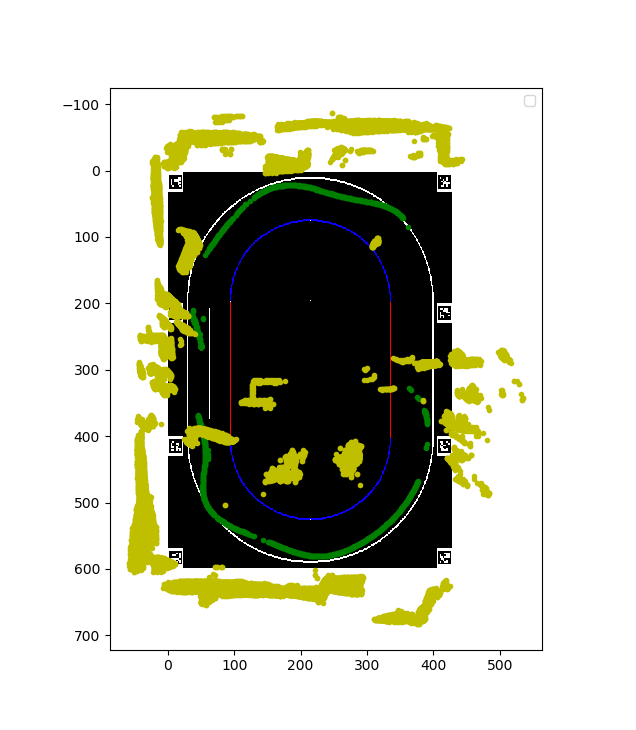
\includegraphics[scale=0.7]{pictures/circle_with_car_and_obstacles.png}
      \caption{Karte mit Lokalisationen des Autos (grün) und erkannte Objekte des LIDARs (gelb). }
    \end{figure}
    \begin{itemize}
      \item Quellcode: \url{https://github.com/bigzed/model_car/blob/version-4.0/texinput/src/localization.py}
      \item Video: \url{https://github.com/bigzed/model_car/blob/version-4.0/texinput/videos/U11_video2.MP4}
    \end{itemize}

	  Der LIDAR erkennt alle Objekte innerhalb von 1.5 m vor dem Auto. Dies umfasst alle Punkte,
    die eine positive X-Koordinate im `laser'-Koordinatensystem haben. Die
    LIDAR Daten sind kontinuierlich, allerdings ben"otigt der Algorithmus die Daten der Odometrie
    um sie in ein gemeinsames Koordinatensystem zu transformieren.

    Wie man an den fehlenden gr"unen Punkten im Plot erkennen kann, hat das Positionssystem
    teilweise lange Verz"ogerungen und es kann auch zum kompletten Ausfall einer Kamera w"ahrend
    einer Fahrt kommen. In der abgebildeten Fahrt fiel wohl die mittlere Kamera aus, was durch
    einen Neustart behoben werden konnte.

    Das Auto ist in dieser Fahrt ungef"ahr an Koordinate $(80 | 400)$ losgefahren und hat die
    Strecke gegen den Uhrzeigersinn befahren. Auf der rechten Geraden erkennt man die
    Ausweichbewegung beginnend etwa bei $(400 | 400)$ um das Hindernis und auf der oberen H"alfte
    der linken Geraden etwa bei $(60 | 280)$ das Stoppen vor dem Hindernis auf beiden Spuren.

    Zu beachten ist, dass die anscheinend komplette Blockade beider Spuren auf der rechten Geraden
    durch ein nachtr"agliches Verschieben des Hindernisses von der inneren auf die "aussere Spur
    entstanden ist, w"ahrend das Auto sich bereits in der nachfolgenden Kurve befand.
    Der LIDAR-Plot ist daher an dieser Stelle irref"uhrend.
	\begin{enumerate}
    \item Für die Transformation benutzen wir \emph{tf.transformations} mit
        \emph{TransformBroadcaster} und \emph{sendTransform} und \emph{TransformListener} sowie
        \emph{transformPoint}. Die LIDAR Daten werden dann in eine \emph{PointCloud2} umgewandelt
        und durch die Transformation in das Koordinatensystem der Odomotetrie "ubertragen.
    \item Wir benutzen die Funktion \emph{closest\_point()} von Übungsblatt 10 mit einigen
        "Anderungen an der Funktion f"ur die Bereiche im Kreis und einem geringen Distanzwert von
        0.3 m.\\
        Der Lenkeinschlag wird aus den Winkeln zwischen Orientierung des Autos (yaw) und dem
        Vektor vom Auto zum \emph{closest\_point} bestimmt. Diesen Winkel nehmen wir als Fehler
        f"ur einen PD-Controller welcher den Lenkwinkel bestimmt.
    \item In unserer \emph{lane\_is\_free} Funktion wird f"ur jedes erkannte Hindernis
        des LIDARs getestet ob es auf der derzeitigen Spur liegt. Falls nicht wird die Spur
        beibehalten. \\
        Falls ein Hindernis auf dieser Spur ist "uberpr"uft der Algorithmus die andere Spur und
        das Auto wechselt die Spur, wenn diese frei ist. Sollte diese ebenfalls belegt sein hält es
        an, bis eine der Spuren wieder frei wird.
	\end{enumerate}
\end{document}
